\vpage{27}{What the extended developments add}{PART II / REPRESENTATION BECOMES CONDITIONAL RECOVERY}{Extension source: precise traditional locators are supplied at final assembly.}
The first twenty-six pages follow the corrected twenty-result formal core. The traditional paper's second part restores the broader mathematical developments of the earlier expanded manuscript. The next thirteen worked pages make their additional hypotheses and conclusions visible.
\head{Four transitions, with the missing input made explicit}
\begin{tabularx}{\linewidth}{@{}p{.21\linewidth}YY@{}}\toprule
Transition & Additional input & Resulting control\\\midrule
Residues to lattices & A finite-index sublattice and one representative per coset & Exact addresses in several dimensions\\
Invertibility to stability & Positive lower frame bound and bounded perturbation & Quantified coefficient and reconstruction error\\
Known jumps to recovery & Separated jumps, sampling, a Lipschitz background, and a strict contrast gap & Exact jump cells and bounded location/amplitude error\\
Recovered packets to approximation & A bounded linear approximation operator and its norm & A complete two-term error estimate\\\bottomrule
\end{tabularx}
\head{The two parts have different formal evidence}
The inherited Lean map covers the twenty designated results of Part I through its 225 supporting targets. The additional traditional proofs in Part II are not silently included in that map. The new pages below are mathematical explanations and exact worked specializations of those developments, with a separate finite-example checker.
The original manuscript's broad edge-recovery questions remain broader than separated one-dimensional jumps. Conditions such as one jump per sample cell, an available wavelet support, and a positive detection margin do real work. In particular, the ambiguous observation on V--19 still rules out an unrestricted recovery guarantee at its stated noise radius.
\head{How to read the extension}
V--28 to V--30 extend coordinates and stability. V--31 to V--34 identify what a singular packet contains and measure its error. V--35 to V--39 give three detection mechanisms. V--40 closes the route by combining packet accuracy with a specified approximation operator.
\takeaway{A positive recovery theorem can coexist with an impossibility example. Their sampling models, noise bounds, and signal classes decide which conclusion applies.}

\vpage{28}{Six image phases are six exact address classes}{LATTICE COORDINATES / A RECTANGULAR EXAMPLE}{Extension source: exact lattice decomposition and refinement.}
Take $L=2\ZZ\times3\ZZ$ inside $\ZZ^2$, with representatives
\[
R=\{0,1\}\times\{0,1,2\}.
\]
Every address has a unique expression $(i,j)=(r_1,r_2)+(2q_1,3q_2)$. The six channels are $x_r(2q_1,3q_2)=x(r_1+2q_1,r_2+3q_2)$.
\vfig[.80]{ext_lattice}
\captiontext{Each cell shows its residue label. Colors identify six disjoint classes; they do not average neighboring image pixels.}
\head{A negative address is still unique}
The point $(-1,7)$ has representative $(1,1)$ and lattice displacement $(-2,6)$, hence channel index $(-1,2)$. Floor division gives the correct answer in both coordinates.
For finite $p$, the channel norm uses the sum of the $p$th powers. At $p=\infty$, it uses their maximum. Both equal the norm on the original lattice because the cosets partition all addresses. In $\ell^\infty$, this coordinate identity does not imply that translates of an impulse are dense: their closure is only $c_0$.
\head{Refinement partitions a class again}
For $L'=4\ZZ\times6\ZZ\subset L$, the coarse representative $(1,2)$ has fine representatives
\[
(1,2),\ (3,2),\ (1,5),\ (3,5).
\]
Their original-lattice masks sum to the coarse mask. As on V--4, decimated arrays are interleaved, not added entrywise.
\takeaway{Dimension changes the address tuple. Unique coset decomposition still supplies exact synthesis and the correct norm identity.}

\vpage{29}{A positive singular-value gap survives perturbation}{FRAME STABILITY / AN EXACT TWO-CHANNEL BANK}{Extension source: imperfect reconstruction, frame bounds and perturbation.}
Consider the constant analysis bank
\[
E=\begin{pmatrix}1&0\\0&2\end{pmatrix},\qquad
E^*E=\operatorname{diag}(1,4).
\]
It has frame bounds $A=1$, $B=4$. For every perturbation with operator norm at most $\delta=1/4$, the squared-norm bounds remain at least $(1-1/4)^2=9/16$ and at most $(2+1/4)^2=81/16$.
\vfig[.87]{ext_frame}
\head{Both bounds can be attained}
Choose $\Delta E=\operatorname{diag}(-1/4,1/4)$. Then $\widetilde E=\operatorname{diag}(3/4,9/4)$ has precisely those two frame bounds. Its inverse has operator norm $4/3$. A coefficient error $\nu=(3/4,0)$ therefore produces signal error $(1,0)$, attaining the noise bound.
The strict condition $\delta<\sqrt A$ prevents the lower bound from vanishing. At $\delta=1$, the perturbation $\operatorname{diag}(-1,0)$ destroys the first channel entirely.
\head{An inverse and an approximate inverse answer different questions}
If the original synthesis $R=\operatorname{diag}(1,1/2)$ is retained after this perturbation, then
\[
R\widetilde E-I=\operatorname{diag}(-1/4,1/8).
\]
Its defect norm is $1/4$. Every input has relative reconstruction error at most that value, with equality on the first coordinate. For frequency-dependent banks the theorem uses an essential supremum on the unit circle, not a few sampled frequencies.
\takeaway{A lower singular-value gap quantifies stable recovery. A reconstruction defect quantifies the error of the actual synthesis bank being used.}

\vpage{30}{Nonunitary tree bounds propagate along branches}{LOCAL FRAME CONSTANTS / A MIXED-DEPTH CERTIFICATE}{Extension source: bounds for nonunitary local splits.}
Suppose the root split has nonnegative squared-norm bounds $A=1/2$ and $B=2$. Retain the left child. Split the right child with bounds $3/4$ and $5/4$, then retain both grandchildren.
\vfig[.85]{ext_tree}
\head{Start with one at every retained node}
The left subtree has bounds $a_0=b_0=1$. The right subtree has $a_1=3/4$ and $b_1=5/4$. The recursive certificate gives
\[
a_{\rm root}=\tfrac12\min\{1,\tfrac34\}=\tfrac38,
\qquad
b_{\rm root}=2\max\{1,\tfrac54\}=\tfrac52.
\]
Consequently the total leaf coefficient energy lies between $3/8$ and $5/2$ times the root energy. These are guaranteed bounds; no assertion that every admissible collection of local maps attains both constants is needed.
\head{Why a minimum and maximum appear}
After the root split, its energy may distribute unevenly between the two children. The lower estimate must survive the least favorable child lower bound. The upper estimate must survive the largest child upper bound. Replacing these by an unweighted average would presume an energy distribution that the hypotheses do not supply.
When all local maps are unitary, every factor is one and the recursion recovers exact energy conservation. For general local maps, a positive lower bound alone establishes injectivity and stable inversion on the range; it does not by itself assert surjectivity onto every possible leaf tuple.
\takeaway{Exact tree coverage and good conditioning are separate inputs. The first chooses a coordinate route; the second bounds what that route does to norms.}

\vpage{31}{Derivative jumps have their own packets}{TRACE DATA / A STEP AND A RAMP}{Extension source: higher-order singular packet decomposition and uniqueness.}
On $[0,1]$, let $H_\tau=\mathbf1_{[\tau,1]}$ and take
\[
f(t)=t^2+2H_{1/3}(t)-3(t-2/3)_+.
\]
The function has a value jump $2$ at $1/3$ and a first-derivative jump $-3$ at $2/3$. Its packet and remainder are
\[
j_f(t)=2\phi_{0,1/3}(t)-3\phi_{1,2/3}(t),\qquad s_f(t)=t^2.
\]
\vfig[.92]{ext_trace}
\captiontext{The displayed curves are exact polynomial pieces. The solid jump is not connected across its discontinuity. The dashed curve is the global smooth remainder.}
\head{The normalization makes the trace coefficient literal}
The general packet is $\phi_{m,\tau}(t)=(t-\tau)_+^m/m!$. Its derivative of order $m$ has a unit trace jump, while its other classical trace jumps vanish. Thus its multiplier is exactly the jump being removed, with no hidden factorial.
Here the remainder has matching value and first-derivative traces and belongs to $W^{2,p}(0,1)$ for every $1\le p\le\infty$. Its second weak derivative is $2$. The singular packet accounts for the distributional boundary terms that would otherwise arise at the breakpoints.
\head{What the general theorem requires}
Each piece must lie in the stated Sobolev class and possess the specified one-sided traces. Subtracting the finite trace packet then joins those pieces into a global Sobolev remainder. This is a theorem about finitely many declared breakpoints, not a representation of every possible singular measure or arbitrary image boundary.
\takeaway{A value jump uses a step. A slope jump uses a ramp. The derivative order determines the packet and its normalization.}

\vpage{32}{The approximation operator also acts on packet error}{ESTIMATED PACKETS / AN EXACT AMPLIFICATION EXAMPLE}{Extension source: reconstruction with an estimated packet.}
Let $Q$ be a bounded \emph{linear} operator and set $e=j-\widehat j$. Substituting $f=s+j$ into $\widehat f=Q(f-\widehat j)+\widehat j$ gives
\[
f-\widehat f=(I-Q)s+(I-Q)e.
\]
The second term includes the action of $Q$ on the packet error. Linearity is required for this split.
\vfig[.80]{ext_amplification}
\head{An oblique projection can increase the error}
In $\RR^2$, choose
\[
Q=\begin{pmatrix}1&2\\0&0\end{pmatrix},\qquad
s=(1,0),\qquad e=(0,1).
\]
Then $Q^2=Q$ and $Qs=s$, but $(I-Q)e=(-2,1)$. The smooth error is zero while the unit packet error becomes a reconstruction error of norm $\sqrt5$.
For a fully specified realization, take $j=e$ and $\widehat j=0$. Then $f=(1,1)$, $\widehat f=Qf=(3,0)$, and their difference is exactly $(-2,1)$.
\head{Use the actual operator bound}
The always-valid estimate in this setting is
\[
\|f-\widehat f\|\leq\|s-Qs\|+(1+\|Q\|)\|e\|.
\]
Here $\|Q\|=\sqrt5$, so the bound is conservative. For an orthogonal projection, $\|I-Q\|\le1$ gives a sharper estimate. The operator's geometry determines which bound can be used.
\takeaway{Recovering the packet and approximating the background are separate tasks, but the chosen approximation operator couples their final errors.}

\vpage{33}{An overlap matrix is an exact error ledger}{REGION VALUES / EVERY MISCLASSIFICATION HAS A WEIGHT}{Extension source: scalar region and overlap matrix formulas.}
Let two piecewise-constant signals have region values $a=(0,2,5)$ and $b=(0,2,5)$ on a counting-measure domain of twelve samples. Suppose their overlap counts are
\[
M=\begin{pmatrix}3&1&0\\0&2&1\\1&0&4\end{pmatrix}.
\]
The row totals $(4,3,5)$ are the true region sizes. The column totals are also $(4,3,5)$, although three samples are assigned to the wrong values.
\vfig[.80]{ext_overlap}
\head{Equal error counts need not mean equal reconstruction error}
The three off-diagonal entries contribute one sample each. Their value differences have magnitudes $2$, $3$, and $5$, so
\[
\|j-\widehat j\|_1=2+3+5=10,\qquad
\|j-\widehat j\|_2^2=4+9+25=38.
\]
The counting-measure supremum error is $5$. The full-domain mean squared error is $38/12=19/6$. A mismatch fraction of $3/12$ reports a different statistic and omits all three amplitude weights.
\head{The formula requires partitions}
For measurable partitions $(E_i)$ and $(F_j)$, with $M_{ij}=\mu(E_i\cap F_j)$,
\[
\|j-\widehat j\|_p^p=\sum_{i,j}|a_i-b_j|^pM_{ij},\qquad 1\le p<\infty.
\]
Each location belongs to exactly one intersection. Overlapping indicator packets that are summed at the same location must first be converted to their actual combined value regions before this partition formula is applied.
\takeaway{Geometry supplies the overlap counts. Signal values supply the weights. Their combination gives the norm relevant to reconstruction.}

\vpage{34}{A shifted step and a shifted ramp have different moduli}{LOCATION STABILITY / A ONE-SIXTEENTH DISPLACEMENT}{Extension source: step location error, higher-order location stability and tube control.}
Set $\tau=1/4$, $\widehat\tau=5/16$, and $\delta=1/16$. A unit step differs only on the interval between its two locations:
\[
\|H_\tau-H_{\widehat\tau}\|_2=\sqrt\delta=\tfrac14,
\qquad \|H_\tau-H_{\widehat\tau}\|_\infty=1.
\]
\vfig[.89]{ext_location}
\head{For a ramp, the error height shrinks too}
Write $r_\tau(t)=(t-\tau)_+$. The difference grows linearly from zero to $\delta$ on $[\tau,\widehat\tau]$ and stays at $\delta$ on $[\widehat\tau,1]$. Direct integration gives
\[
\|r_\tau-r_{\widehat\tau}\|_2^2
=\frac{\delta^3}{3}+(1-\widehat\tau)\delta^2
=\frac{17}{6144}<\frac1{256}=\delta^2.
\]
Thus the $L^2$ ramp error is at most $\delta$, and its supremum error is exactly $\delta$. Positive-order truncated powers are Lipschitz in location, with the order-dependent constants supplied by the theorem.
\head{The geometric analogue needs a tube hypothesis}
If $E\triangle F\subseteq N_\delta(\partial E)$ and the tube measure is bounded by $C\delta$ for the stated range $0<\delta<\delta_0$, then an equal-amplitude packet has finite-$p$ error at most $|a|(C\delta)^{1/p}$. A mere visual impression that two boundaries are close does not establish the inclusion or the tube estimate.
\takeaway{A displaced value jump keeps its full height on a smaller set. A displaced derivative-jump packet also decreases in height.}

\vpage{35}{A strict contrast gap locates every separated jump cell}{DETERMINISTIC RECOVERY / A NUMERICAL CERTIFICATE}{Extension source: contrast gap and deterministic jump-cell recovery.}
Assume a real signal is a Lipschitz background plus jumps. No jump occurs at a sample point, and each grid cell contains at most one jump. With spacing $h$, background constant $M$, and sample noise bounded by $\varepsilon$, write
\[
b_h=Mh+2\varepsilon.
\]
A no-jump contrast has magnitude at most $b_h$. A jump contrast differs from its true amplitude by at most $b_h$.
\vfig[.89]{ext_threshold}
\head{Use the manuscript's exact numerical inputs}
For $h=1/256$, $M=1/2$, $\varepsilon=1/500$, and $a_{\min}=2/25$,
\[
b_h=\frac{381}{64000}<\frac3{500},\qquad
2b_h<\frac2{25}.
\]
The threshold $\theta=1/25$ lies strictly between $b_h$ and $a_{\min}-b_h$. Thresholding $|y_{k+1}-y_k|$ therefore identifies exactly the jump-containing cells. Their midpoints locate each jump within $1/512$, and each estimated amplitude differs by at most $381/64000$.
\head{The recovered object is a cell, then an estimate}
The theorem does not claim the exact real-valued breakpoint from a finite grid. It supplies the correct cell and a controlled representative of that cell. For real jumps, the amplitude error is too small to reverse the sign. Two opposite jumps in one cell could cancel in the contrast, which is why the separation assumption cannot be dropped.
For $Q$ jumps the finite-$p$ packet bound contains both $Qb_h$ and the location term $(\tfrac h2\sum_q|a_q|^p)^{1/p}$. A growing number of jumps or shrinking separation requires its own analysis.
\takeaway{Exact detection means exact cell identification under a strict margin. Location and amplitude remain quantitative estimates with explicit errors.}

\vpage{36}{Repeated observations shrink the noise side of the gap}{SUBGAUSSIAN RECOVERY / A CONSERVATIVE SAMPLE BUDGET}{Extension source: probability recovery and repeated measurements.}
Suppose all noise observations are independent and centered, with moment-generating bound $\mathbb E e^{\lambda\eta}\le e^{\sigma^2\lambda^2/2}$. Averaging $R$ observations at each of $n+1$ sample sites replaces $\sigma$ by $\sigma/\sqrt R$. A sufficient recovery condition is
\[
a_{\min}>2Mh+\frac{4\sigma}{\sqrt R}\sqrt{\log(2n/\delta)}.
\]
The probability of simultaneous recovery is then at least $1-\delta$, subject to the same separated-jump sampling model.
\vfig[.86]{ext_repetition}
\head{One explicit conservative choice}
Take $n=256$, $M=1/2$, $\sigma=1/50$, $\delta=1/20$, and $a_{\min}=2/25$. Since $\log(10240)<10<(16/5)^2$, choosing $R=16$ makes the right-hand side strictly less than
\[
\frac1{256}+\frac1{50}\frac{16}{5}
=\frac{2173}{32000}<\frac2{25}.
\]
Thus sixteen independent observations per sample site suffice for this bound. It is a sufficient budget, not a claim of optimal sample complexity. The exact checker certifies $e^{10}>10240$ using a rational Taylor partial sum, so the displayed logarithm bound is not based on rounded numerical logarithms.
\head{Dependence between adjacent contrasts is allowed}
Neighboring differences share one sample. The proof does not require those differences to be independent: it bounds each tail and applies a union bound across all cells. Independence of the underlying sample noises supplies the stated subGaussian difference proxy.
For a fixed separated signal model, a noise scale satisfying $\sigma_n\sqrt{\log n}\to0$ gives the stated recovery consistency in probability. A fixed positive noise scale with one observation per site does not satisfy that condition.
\takeaway{More grid points and more repeated observations affect different terms. Finer spacing reduces background variation; averaging reduces noise.}

\vpage{37}{Haar sees a jump only through its position in the support}{SCALE SEPARATION / A QUANTIFIED THRESHOLD}{Extension source: smooth Haar bound and exact step coefficient.}
Use a normalized Haar wavelet on an available interval of length $L$ on the real line, positive on its left half and negative on its right half. Here $H_\tau$ is the half-line step $\mathbf1_{[\tau,\infty)}$, so there is no artificial second endpoint jump.
If $u$ is the relative jump position in the support, then
\[
|\langle aH_\tau,\psi\rangle|
=|a|\sqrt L\min\{u,1-u\}.
\]
The coefficient vanishes when the jump lies exactly at a support boundary.
\vfig[.86]{ext_haar_margin}
\head{A worked gap with all three contributions}
Take $L=1/4$, $M=1$, noise bound $\varepsilon=1/100$, jump size $|a|=1$, and relative boundary distance at least $\rho=1/4$. The smooth and noise contributions together are bounded by
\[
\frac M4L^{3/2}+\varepsilon\sqrt L
=\frac1{32}+\frac1{200}=\frac{29}{800}.
\]
The jump contributes at least $|a|\rho\sqrt L=1/8$. The observed coefficient therefore has magnitude at least $71/800$. The threshold $1/16=50/800$ separates every such jump support from every support containing no jump.
\head{The available support is part of the hypothesis}
A fixed extension is needed if the observation domain ends inside a desired wavelet support. Also, the selected support must contain only the specified jump. An unmodeled second jump can reinforce or cancel the coefficient.
\takeaway{Scale determines the smooth contribution, but alignment determines the jump contribution. A detection guarantee needs both.}

\vpage{38}{Two half-shifted grids remove exact alignment failure}{HAAR SUPPORT GEOMETRY / A QUARTER-CELL GUARANTEE}{Extension source: half-cell shift and two-grid detection.}
Normalize the support length to $L=1$. The first grid has boundaries at integers; the second has boundaries at half-integers. For a point at position $u$ modulo one, consider its distance to the nearest boundary of each grid.
\vfig[.89]{ext_two_grids}
\head{At least one distance is one quarter or larger}
If $1/4\le u\le3/4$, the original cell works. Outside that range, a shifted cell works. At $u=1/8$, the original margin is $1/8$ but the shifted cell $[-1/2,1/2)$ gives margin $3/8$. At $u=1/4$, both margins equal $1/4$, showing that the uniform constant cannot be increased for these two grids.
Restoring $L$, every jump has a support with boundary distance at least $L/4$ in one grid. If $L$ is smaller than the minimum jump separation, that support contains no other jump.
\head{Insert the geometric guarantee into the analytic estimate}
The alignment-independent gap condition is
\[
\frac{|a|}{4}>2\varepsilon+\frac M2L.
\]
For the numbers on V--37, the right side is $1/50+1/8=29/200$, strictly below $1/4$. Hence one of the two grids supplies a detectable support for every jump, regardless of its position relative to the original grid.
This certifies a useful support per jump. It does not by itself specify a unique rule for merging duplicate detections from two grids into exact breakpoint estimates.
\takeaway{A second grid repairs a geometric blind spot. The contrast inequality and separation hypotheses still supply the recovery guarantee.}

\vpage{39}{Higher differences annihilate polynomial interiors}{BOUNDARY STENCILS / SIGNAL RESPONSE AND NOISE GAIN}{Extension source: polynomial annihilation and robust breakpoint bands.}
Let $x(n)=n+2(n-3)_+$ on the integer line. Its slope changes from one to three at the breakpoint $3$. The second forward difference is
\[
\Delta^2x(n)=x(n+2)-2x(n+1)+x(n).
\]
\vfig[.87]{ext_differences}
\head{An exact small stencil calculation}
The values at $n=0,\ldots,6$ are $(0,1,2,3,6,9,12)$. The second differences at $n=0,\ldots,4$ are $(0,0,2,0,0)$. The only nonzero stencil straddles the slope change.
For a piecewise polynomial of degree at most $d$, $\Delta^{d+1}$ vanishes whenever its complete stencil lies inside one polynomial piece. Candidate responses are confined to at most $d+1$ starting addresses before each breakpoint. They are boundary bands, not necessarily exact breakpoint locations.
\head{Differencing also acts on noise}
The absolute binomial coefficients of $\Delta^m$ sum to $2^m$. With $\|\eta\|_\infty\le1/16$, second-difference noise is bounded by $4/16=1/4$. The true response $2$ remains at least $7/4$, while all responses away from the breakpoint band remain at most $1/4$. Threshold one separates them.
The general robust-band statement assumes that each breakpoint has at least one sufficiently large true response. A breakpoint can fail that assumption through its amplitude or local configuration. Annihilation away from boundaries does not prove a lower bound at every boundary.
\takeaway{A vanishing interior response is structural. Reliable detection also requires the boundary response to exceed the amplified noise.}

\vpage{40}{Conditional Gibbs control closes the reconstruction estimate}{THE TWO ERRORS / A COMPLETE READING CONTRACT}{Extension source: exact and estimated packet convergence.}
The exact retained-packet approximation shares the same discontinuity as its target. If $f=s+j$ and $Q_ms\to s$ uniformly, then
\[
\|f-(Q_ms+j)\|_\infty=\|s-Q_ms\|_\infty\longrightarrow0.
\]
The approximants themselves may be discontinuous. There is no conflict with the failure of continuous Fourier polynomials to converge uniformly to a jump.
\begin{center}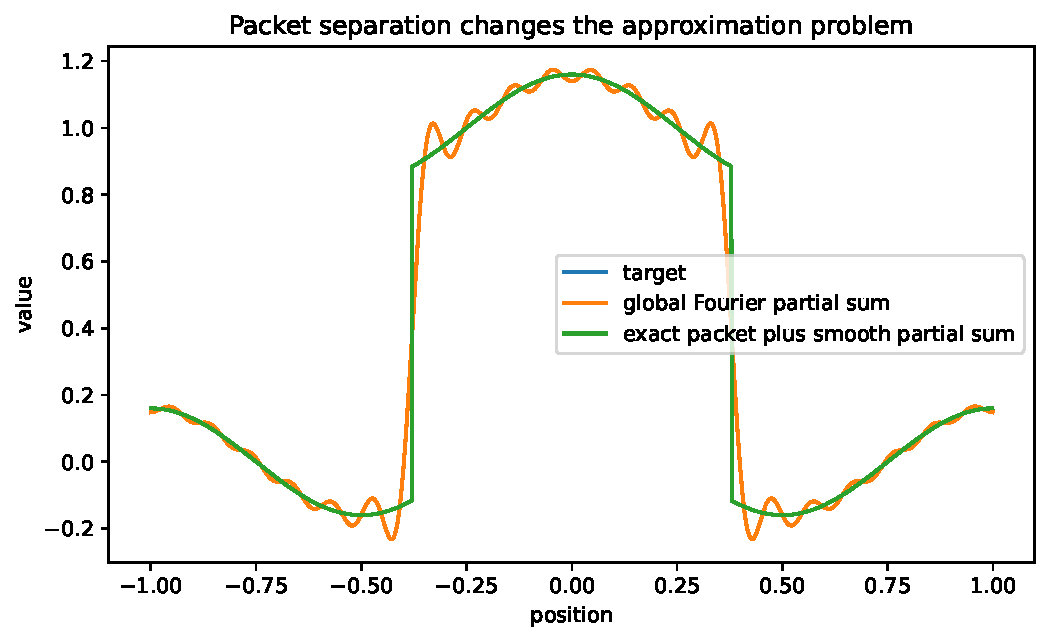
\includegraphics[width=.78\linewidth]{graphics/annals_gibbs_comparison.pdf}\end{center}
\captiontext{Preserved vector figure from the expanded source. It illustrates the choice of approximation target; it is not an independent universal recovery certificate.}
\head{Estimated packets need the operator norm too}
If the bounded linear operators satisfy $\sup_m\|Q_m\|_{L^p\to L^p}\le C_Q$, then
\[
\|f-\widehat f_m\|_p
\le\|s-Q_ms\|_p+(1+C_Q)\|j-\widehat j_m\|_p.
\]
For an orthogonal $L^2$ projection one may use $\|I-Q_m\|\le1$, sharpening the packet multiplier to one. Such a bound must be justified in the norm actually being used. In particular, uniform boundedness of Fourier partial sums in the supremum norm is not supplied by this theorem.
\head{What the complete guide establishes}
V--1 to V--26 preserve the original worked layer. V--27 to V--40 explain the additional traditional developments, outside the inherited twenty-result Lean map. The new exact examples have their own finite arithmetic record. They do not extend the formal coverage merely by appearing beside formally mapped results.
The final package keeps current executions, inherited compiler reports, and unrun suites distinct. The saved visual report of 181 checks and seven invalid controls remains inherited; this edition does not claim that SymPy-dependent suite or Lean was rerun.
\takeaway{A complete error claim specifies the signal class, the recovered packet, the approximation operator, and the norm. Each term can then be improved and checked on its own terms.}
